\documentclass[tikz, border=2mm]{standalone}
\usetikzlibrary{shapes, arrows.meta}

\begin{document}

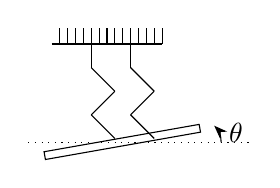
\begin{tikzpicture}
    % Support rod (horizontal)
    \draw (0.8,2) -- (2.2,2); % Shortened the support system

    % First Rectangle
    \draw[rotate=10] (0.8,0.4) rectangle (2.8,0.5);
    
    % First Spring (tight rod)
    \draw (1.6,0.8) -- (1.3,1.1);
    \draw (1.3,1.1) -- (1.6,1.4);
    \draw (1.6,1.4) -- (1.3,1.7);
    \draw (1.3,1.7) -- (1.3,2);
    
    \foreach \i in {1,...,14}
        \draw ({0.8 + 0.1*\i},2) -- ({0.8 + 0.1*\i},2.2);
    
    % Support rod (horizontal)
    \draw (0.8,2) -- (2.2,2); % Shortened the support system
      % Second Spring (tight rod)
    \draw (2.1,0.8) -- (1.8,1.1);
    \draw (1.8,1.1) -- (2.1,1.4);
    \draw (2.1,1.4) -- (1.8,1.7);
    \draw (1.8,1.7) -- (1.8,2);

    \draw[thin, dotted] (0.5,0.75) -- (3.3,0.75);
    \draw[->, >=Stealth] (2.95, 0.75) arc (0:45:0.3) node[midway, right] {$\theta$};
\end{tikzpicture}

\end{document}

